%%%%%%%%%%%%%%%%%%%%%%%%%%%%%%%%%%%%%%%%%%%%%%%%%%%%%%%%%%%%%%%%%%%%%%%%%%%%%%%%
%2345678901234567890123456789012345678901234567890123456789012345678901234567890
%        1         2         3         4         5         6         7         8

% \documentclass[letterpaper, 10 pt, conference]{ieeeconf}  % Comment this line out if you need a4paper

\documentclass[a4paper, 10pt, conference]{ieeeconf}      % Use this line for a4 paper

\IEEEoverridecommandlockouts                              % This command is only needed if 
                                                          % you want to use the \thanks command

\overrideIEEEmargins                                      % Needed to meet printer requirements.

%In case you encounter the following error:
%Error 1010 The PDF file may be corrupt (unable to open PDF file) OR
%Error 1000 An error occurred while parsing a contents stream. Unable to analyze the PDF file.
%This is a known problem with pdfLaTeX conversion filter. The file cannot be opened with acrobat reader
%Please use one of the alternatives below to circumvent this error by uncommenting one or the other
%\pdfobjcompresslevel=0
%\pdfminorversion=4

% See the \addtolength command later in the file to balance the column lengths
% on the last page of the document

% The following packages can be found on http:\\www.ctan.org
\usepackage{graphics}
%\usepackage{parskip} % for pdf, bitmapped graphics files
\usepackage{epsfig} % for postscript graphics files
\usepackage{mathptmx} % assumes new font selection scheme installed
\usepackage{times} % assumes new font selection scheme installed
\usepackage{amsmath} % assumes amsmath package installed
\usepackage{amssymb}  % assumes amsmath package installed
\usepackage{float}

\title{\LARGE \bf Implementation of biologically-inspired dynamical systems for movement generation: automatic real-time goal adaptation and obstacle avoidance}

\author{Alan Gomez, Samuel Parra, and Brennan Penfold}
\setlength{\parskip}{0pt}

\begin{document}



\maketitle
\thispagestyle{empty}
\pagestyle{empty}


%%%%%%%%%%%%%%%%%%%%%%%%%%%%%%%%%%%%%%%%%%%%%%%%%%%%%%%%%%%%%%%%%%%%%%%%%%%%%%%%
\begin{abstract}


\end{abstract}


%%%%%%%%%%%%%%%%%%%%%%%%%%%%%%%%%%%%%%%%%%%%%%%%%%%%%%%%%%%%%%%%%%%%%%%%%%%%%%%%
\section{Introduction} %Brennan
% Background, motivation and state of the art

%Background ---------------
Humanoid robots and arm like manipulators have a great many current, and potential, useful applications. Currently robotic manipulators are used in a range of manufacturing processes like painting and spot welding \cite{Fadalil}. Another great application of humanoid robotics is to help people who cannot help themselves, as a separate system, or as a prosthetic. Currently there are prosthetics available, like Dean Kamen's Luke Arm \cite{Adee}, but the control of such device is limited. In human applications the control system used in areas like manufacturing cannot be just dropped into place there are many considerations that are required from a software and hardware perspective. In manufacturing applications the manipulators typically use precomputed trajectories for robustness and efficiency, but this is unsuitable in a human environment where obstacles and goals are constantly on the move \cite{Hoffmann}. The current approach is to use a human controller to solve this problem by adding a controller in a shoe \cite{Adee} or another such interface. While this addresses the issue is can be quite taxing for the user, requiring a lot of concentration just to perform basic tasks.

A solution to the control problem is to use dynamic movement principles which can be generated during the movement itself, allowing for real-time obastacle avoidance and goal changes. Previous approaches \cite{Janabi-Sharif} used were initially not able to handle moving goals, but improvements made by H. Hoffmann et al. \cite{Hoffmann} by applying a potential field method to the process overcame this limitation. The use of dynamic movement primitives in the potential field method overcame the local minimum problem that is typically inherent with using potential fields. Hence this paper is the basis of the project.

%State of the art -----------
% This paper only considers the end-effector 
% Paper considers the velocity direction and obstacle direction
% Does not consider distance 

For the objects to be avoided first they must be located relative to the manipulator, and that is the core concept of the library built for this project. Biologically-inspired dynamical systems for movement generation \cite{Hoffmann} does not tackle the problem of distances between objects, instead a precursor paper was used, Real-Time Obstacle Avoidance for Manipulators and Mobile Robots \cite{Khatib}. This paper goes into details on how to find the distance between two obstacles, which was modified to find the vector, allowing for it to be applied to the dynamic movements primitives control algorithm discussed in Biologically-inspired dynamical systems for movement generation \cite{Hoffmann}.
%Robotic assistants

\section{Approach}

\subsection{Distance to objects} %Alan
To compute the closest distance between two objects we first obtain the closest points between the objects and then the distance between these two points.

1) Sphere - Sphere: 
To compute the closest distance between two spheres, one can easily calculate the distance between the center of both spheres and subtract the radius of both spheres.

2) Sphere - Capsule:
To compute the closest distance between a capsule $C$ and a sphere $S$, one can compute the distance between the center of $S$ = $p_S$ and the axis of symmetry of $C$ = $l_C$
and then subtract the radius of the sphere and the capsule. 

The closest point, on $l_C$, to $p_S$ is given by \eqref{eq:capsule_point},

\begin{equation}       
    \begin{matrix} 
        x = x_1 + \lambda(x_2 - x_1) \\
        y = y_1 + \lambda(y_2 - y_1) \\
        z = z_1 + \lambda(z_2 - z_1) \label{eq:capsule_point}
    \end{matrix}
\end{equation}

where the start point of $l_C$ is $m1(x_1, y_1, z_1)$, the end point is $m2(x_2, y_2, z_2)$, and $\lambda$ is given by \eqref{eq:lambda}.

\begin{equation}       
    \begin{matrix} 
        \lambda = \frac{(c - m_1) \cdot (m_2 - m_1 )}{l^2} \label{eq:lambda}
    \end{matrix}
\end{equation}

3) Capsule - Capsule:
To compute the closest distance between two capsules (capsule $A$ and capsule $B$), with axis of symmetry $l_A = \overline{m1_A m2_A}$ and $l_B = \overline{m1_B m2_B}$, 
where $A$ is the longest capsule, one can consider four different cases:
\begin{enumerate}
    \item $m1_B$ and $m2_B$ can be perpendicularly projected onto $l_A$
    \item $m1_B$ and $m2_B$ cannot be perpendicularly projected onto $l_A$
    \item only $m1_B$ can be perpendicularly projected onto $l_A$
    \item only $m2_B$ can be perpendicularly projected onto $l_A$
\end{enumerate} 

Depending on these cases, the following steps are going to be calculated with different objects.

In case 1, capsule $M$ will be capsule $A$, and capsule $O$ will be capsule $B$.

In case 2, if $m1_B$ is closer to $l_A$ than $m2_A$ is to $l_B$, then capsule $M$ will be capsule $A$, and capsule $O$ will be capsule $B$.
Else capsule $M$ will be capsule $B$, and capsule $O$ will be capsule $A$.

In case 3, if $m2_B$ is closer to $l_A$ than $m1_A$ is to $l_B$, then capsule $M$ will be capsule $A$, and capsule $O$ will be capsule $B$.
Else capsule $M$ will be capsule $B$, and capsule $O$ will be capsule $A$.

In case 4, if if $m1_B$ is closer to $l_A$ than $m2_B$ is to $l_A$, then capsule $M$ will be capsule $A$, and capsule $O$ will be capsule $B$.
Else capsule $M$ will be capsule $B$, and capsule $O$ will be capsule $A$.

With capsule $M$ and capsule $P$, one can follow the next steps.
The first step is to place the reference frame of $M$ in its center of mass, with the Z-axis in the direction of $l_M$. 
The second step is to project $l_O$ onto the XY-plane given by the reference frame of $M$ (Figure \ref{fig:capsule_capsule}),
the result of this projection would be the line $l_P$.
The third step is to calculate the closest point on $l_P$ to the origin of the reference frame of $P$ by using \eqref{eq:capsule_point}. 
The final step is to compute the distance and subtract the radius of the capsule and the sphere.
If the true closest points on the original axis of symmetry of the capsules are needed, one can project back the obtained points.

\begin{figure}[H]
    \centering
    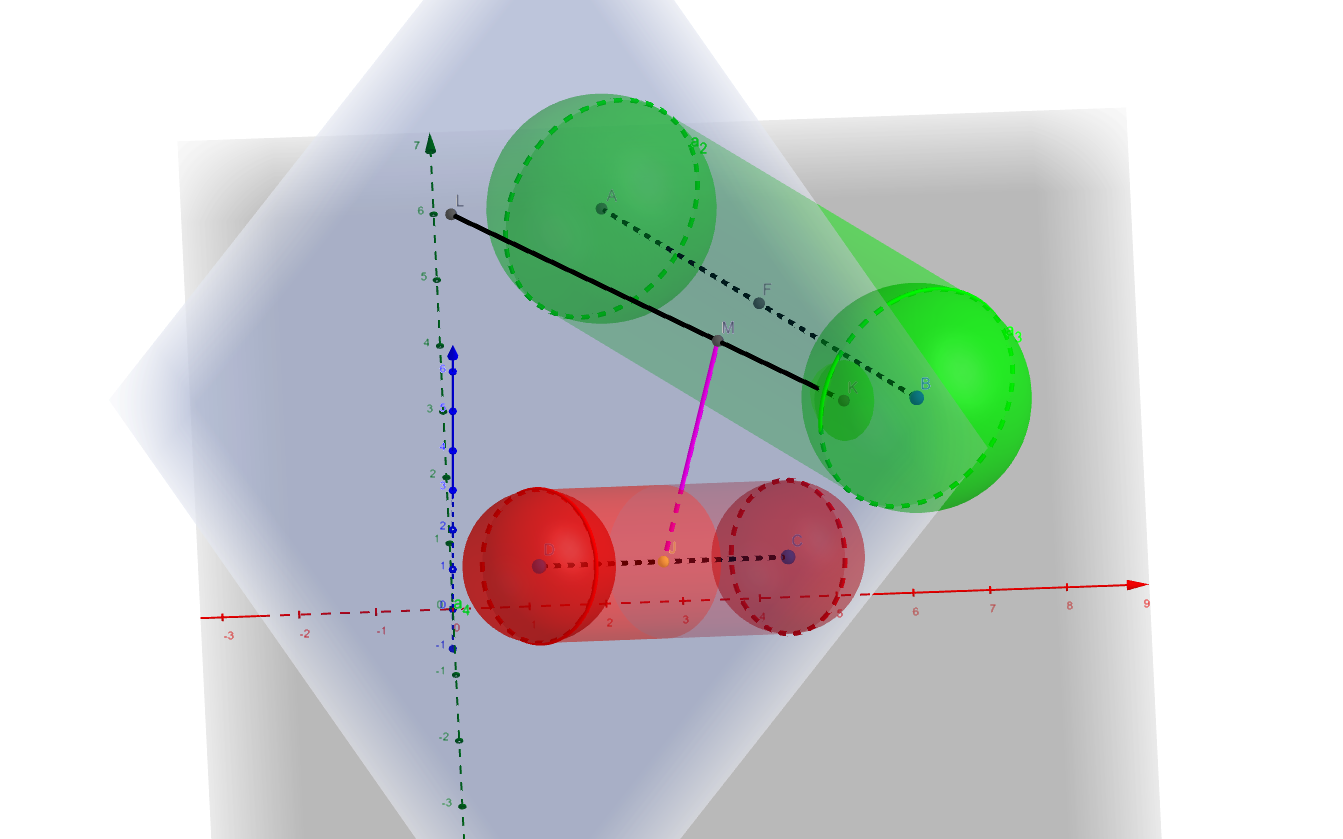
\includegraphics[scale=0.15]{images/capsule-capsule.png}
    \caption{Capsule - capsule}
    \label{fig:capsule_capsule}
\end{figure}


\subsection{Potential field} %Sam

To avoid collisions we decided to implement the method presented in \cite{1}. This method is based on dynamic movement primitives (DMP), which are used to generate a trajectory $x(t)$ with a velocity $v(t)$. These DMP are motivated from the dynamic of damped spring and can generate trajectories in many dimensions. These can be used to describe accelerations in 3D space that move towards a goal:

\begin{equation} \label{eq:1}
	\dot{v} = K ( g - x ) - D v - K (g - x_0) s + K f(s) + p(x, v)
\end{equation}

Where $g$ is the goal, $x$ is the current position, $x_0$ is the starting position, $v$ is the current velocity, $s$ is the phase variable, $D$ is the damping constant, and $K$ is the spring constant. The function $f(s)$ is a nonlinear function used to define a learned path for the manipulator to take. However, the terms dependent on $s$ are not relevant for our application; thus we decided to not include it in the final equation.  

The last term is the potential field generated by the obstacles. This term has a repel effect on the end effector, making it avoid obstacles. The potential field is calculated as follow: We first determine the steering angle $\varphi$ using equation \ref{eq:2}, which is the angle between the velocity vector and a vector from the end effector to the obstacle as seen in Fig \ref{steering_image}. In our implementation, this vector is the shortest distance between the end-effector and the obstacle, as the original method considered points instead of volumes.


\begin{figure}
	\centering
	\scalebox{0.55}{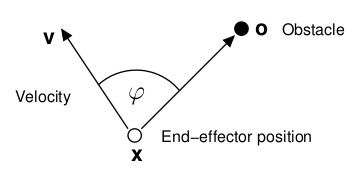
\includegraphics{images/steering_angle.png}}
	\caption{Graphical representation of steering angle \cite{1}}
	\label{steering_image}
\end{figure}

\begin{equation} \label{eq:2}
	\varphi = cos^{-1} ((o-v)^T v / (\|o-x\| \cdot \|v\|));
\end{equation}

This steering angle determines how sharp the end effector steers away from the obstacle. The closer the angle is to 0, the more abrupt is the change of direction. the potential field is given by:

\begin{equation}
	p(x, v) = \gamma \sum_i R_i v \phi_i exp(-\beta \varphi_i) 
\end{equation}

Where $\gamma$ and $\beta$ are constants, and R is a rotation matrix which rotates by the axis $r = (o-x) \times v $ with an angle of rotation of $\pi/2$. This rotation matrix can be calculated with the Rodrigues' rotation formula \cite{rodrigues}. The final potential field is the sum of the potential fields generated by all the obstacles. Our final equation converges towards the goal avoiding the obstacles in its way.

\begin{equation}
\dot{v} = K ( g - x ) - D v + p(x, v)
\end{equation}

\subsection{Collision monitoring library} %Sam

Our library was designed to be platform and framework independent. To achieve this, the library user must implement the Arm interface. This provides the flexibility of choosing how to describe mathematically the manipulator and update its position. Consider the case of two developers, one wants to use KDL for the forward and backwards kinematics, while the other one wants to derive the equations manually for a closed form solution. Both developers are supported by this library. 

In order to monitor the distances from the links of the arm to the obstacles in the workspace we represent the geometry of the links with the use of capsules. This representation enables us to calculate the distances between the links themselves in order to monitor self-collisions along with regular obstacles. This requires that the developer updates the geometric representation alongside the arm’s movement in the Arm implementation. 


\subsection{Controller} %Sam

The manipulator is controlled with a control loop that is executed at a specified rate. This loop is responsible for updating the geometric representation to match the real life manipulator and calculate the new velocity with the collision avoidance algorithm. In the loop the developer must keep the current position, velocity, positions of obstacles, and goal updated for the algorithm to produce an accurate output. 
 
\section{Implementation} %Brennan
\subsection{ROS} %Brennan
%  Purpose of ROS Implementations
% Layout of code
% Control algorithim
% Simulation of manipulator
% 
\subsection{Results} %Brennan
% Performance of collsision monitoring
% - timing stress test
% Performance of obstacle avoidance
% - graphs of avoidance
% - ROS update rate
% Features
% Deficits
% improvemnts/future works

\section{Experiments}

\subsection{Collision Monitoring} %Brennan

\subsection{Single arm avoidance} %Sam

\subsection{Dual arm avoidance} %Sam


\section{Use case}

\subsection{Single arm} %Alan
The library presented in this paper can be used with a single manipulator to avoid the collision of its end-effector with objects in the environment.
The user can use the Arm interface to provide the necessary information about the manipulator.
The user can then also add different obstacles that are present in the environment.
The pose of the manipulator and the obstacles need to be updated using the methods given by the library.
\subsection{Dual arm} %Alan
One can also use the library with two manipulators by creating two instances of the implementation of the Arm interface and adding the links of 
the opposite manipulator as obstacles represented by capsules.
This will prevent the collision of the end-effector of both robots with the opposite manipulator
\subsection{Multiple arms}
In the same way, as one can use the library with two manipulators, one can add as many manipulators as the computational resources allow it.
\subsection{Self collision} %Alan
Finally, one can also use this library to prevent the collision of the end-effector of the manipulator with its other links.
This can be done by implementing the Arm interface and adding each link of the robot as an obstacle represented by a capsule.

\section{Conclusion} %Alan
The computation of the distances between different kinds of objects is not easy, one needs to take into consideration different scenarios, 
otherwise, the main algorithm might fail. Further work on this area could be adding other kinds of shapes.


\addtolength{\textheight}{-12cm}   % This command serves to balance the column lengths
                                  % on the last page of the document manually. It shortens
                                  % the textheight of the last page by a suitable amount.
                                  % This command does not take effect until the next page
                                  % so it should come on the page before the last. Make
                                  % sure that you do not shorten the textheight too much.

%%%%%%%%%%%%%%%%%%%%%%%%%%%%%%%%%%%%%%%%%%%%%%%%%%%%%%%%%%%%%%%%%%%%%%%%%%%%%%%%



%%%%%%%%%%%%%%%%%%%%%%%%%%%%%%%%%%%%%%%%%%%%%%%%%%%%%%%%%%%%%%%%%%%%%%%%%%%%%%%%



%%%%%%%%%%%%%%%%%%%%%%%%%%%%%%%%%%%%%%%%%%%%%%%%%%%%%%%%%%%%%%%%%%%%%%%%%%%%%%%%
\section*{Appendices}

\section*{Acknowledgments}


%%%%%%%%%%%%%%%%%%%%%%%%%%%%%%%%%%%%%%%%%%%%%%%%%%%%%%%%%%%%%%%%%%%%%%%%%%%%%%%%


\begin{thebibliography}{99}

\bibitem{Fadalil} M. S. Fadali and A. Visioli, “Introduction to Digital Control,” in Digital Control Engineering, Elsevier, 2013, pp. 1–8.


\bibitem{Hoffmann} H. Hoffmann, P. Pastor, D.-H. Park, and S. Schaal, “Biologically-inspired dynamical systems for movement generation: Automatic real-time goal adaptation and obstacle avoidance,” in 2009 IEEE International Conference on Robotics and Automation, Kobe, May 2009, pp. 2587–2592, doi: 10.1109/ROBOT.2009.5152423.
\bibitem{Velliste} M. Velliste, S. Perel, M. C. Spalding, A. S. Whitford, and A. B. Schwartz, “Cortical control of a prosthetic arm for self-feeding,” Nature, vol. 453, no. 7198, Art. no. 7198, Jun. 2008, doi: 10.1038/nature06996.
\bibitem{Adee} S. Adee, “Dean Kamen’s ‘Luke Arm’ Prosthesis Readies for Clinical Trials - IEEE Spectrum,” IEEE Spectrum: Technology, Engineering, and Science News, Feb. 01, 2008. https://spectrum.ieee.org/biomedical/bionics/dean-kamens-luke-arm-prosthesis-readies-for-clinical-trials (accessed Jun. 25, 2020).
\bibitem{Janabi-Sharif} F. Janabi-Sharifi and D. Vinke, “Integration of the artificial potential field approach with simulated annealing for robot path planning,” in Proceedings of 8th IEEE International Symposium on Intelligent Control, Aug. 1993, pp. 536–541, doi: 10.1109/ISIC.1993.397640.
\bibitem{Khatib} O. Khatib, “Real-Time Obstacle Avoidance for Manipulators and Mobile Robots” The International Journal of Robotics Research, vol. 5, no. 1, pp. 90–98, Mar. 1986, doi: 10.1177/027836498600500106.
\bibitem{rodrigues}  Belongie, Serge. "Rodrigues' Rotation Formula." From MathWorld--A Wolfram Web Resource, created by Eric W. Weisstein. https://mathworld.wolfram.com/RodriguesRotationFormula.html 



\end{thebibliography}


\end{document}
